\documentclass[tikz]{standalone}
\usetikzlibrary{calc}
\usepackage{pgfplots}
\usepgfplotslibrary{polar}
\pgfplotsset{compat=1.9}

\begin{document}
   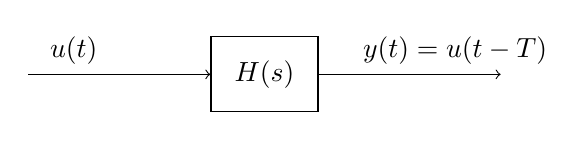
\begin{tikzpicture}[node distance=30mm, anchor=north]
   \node[coordinate] (input) {};
   \node[rectangle, draw, right of=input, inner sep=3mm] (lti) {$H(s)$};
   \node[coordinate, right of=lti] (output) {};
   \draw[->] (input) -- node[near start, above] {$u(t)$}  (lti);
   \draw[->] (lti) -- node[near end, above] {$y(t)=u(t-T)$} (output);
   \end{tikzpicture}
\end{document}
